\documentclass[conference]{IEEEtran}
\usepackage{cite}
\usepackage{amsmath,amssymb,amsfonts}
\usepackage{graphicx}
\usepackage{textcomp}
\usepackage{xcolor}
\usepackage{url}
\usepackage{booktabs}

\begin{document}

\title{Task [C1]: [English-to-Urdu Neural Machine Translation]}

\author{\IEEEauthorblockN{Muhammad Zaryab Attiq}
\IEEEauthorblockA{Roll No. 70176119 \quad Section A\\
Repository: \url{https://github.com/Vex456/AI101-ML-Assignment-70176119}\\
Instructor: Dr. Muhammad Awais, AI Architect}
}

\maketitle

\section{Introduction}
Neural Machine Translation (NMT) maps variable-length sequences from a source language to a target language via parameterized deep neural networks. Translating English into Urdu is challenging due to structural, morphological, and orthographic asymmetries: English exhibits rigid Subject-Verb-Object (SVO) syntax with Latin left-to-right orthography, whereas Urdu features Subject-Object-Verb (SOV) order, flexible scrambling, and complex verbal agreement written right-to-left in the Perso-Arabic script. Furthermore, Urdu remains low-resource in curated parallel text. In this study, we build an attention-augmented Sequence-to-Sequence (Seq2Seq) model from scratch using a Bidirectional GRU encoder and Bahdanau additive cross-attention. We evaluate greedy search versus beam search ($k=4$) and benchmark against a pretrained Transformer (MarianMT). Our findings demonstrate that beam search achieves a 52.2\% relative gain in BLEU over greedy search, while cross-attention dynamically bridges the structural gap between English SVO and Urdu SOV word order.

\section{Problem Statement}
Given a source English token sequence $X = (x_1, \dots, x_T)$, the goal is to model the conditional probability distribution over target Urdu sequences $Y = (y_1, \dots, y_{T'})$:
\begin{equation}
P(Y \mid X) = \prod_{t=1}^{T'} P(y_t \mid y_{<t}, X)
\end{equation}
Model parameters $\theta$ are trained using token-level Cross-Entropy Loss with teacher forcing, masking padding tokens:
\begin{equation}
\mathcal{L}(\theta) = - \sum_{t=1}^{T'} \log P_\theta(y_t^* \mid y_{<t}^*, X)
\end{equation}
At inference time, target sentences are decoded either via greedy argmax selection or beam search ($k=4$) with length normalization $\frac{1}{t^\alpha} \sum_{\tau=1}^t \log P(y_\tau \mid y_{<\tau}, X)$. Evaluation is conducted on held-out test data using standardized \texttt{sacreBLEU} and character n-gram F-score (\texttt{chrF}).

\section{Dataset Used}
We employ the OPUS-100 English-Urdu (\texttt{en-ur}) corpus from Helsinki-NLP~\cite{tiedemann2012}. The raw corpus contains 753,913 training pairs, 2,000 validation pairs, and 2,000 test pairs. Because web-mined text contains substantial misalignment and corrupt encodings, we enforce a strict 5-stage cleaning pipeline: (1) removal of empty strings, (2) deduplication (29,505 duplicate pairs removed), (3) target script verification ensuring characters in Unicode range \texttt{\textbackslash u0600}--\texttt{\textbackslash u06FF} (1,510 pairs dropped), (4) length filtering capping source and target at 30 whitespace tokens (288,649 pairs dropped), and (5) length ratio filtering capping length divergence at 3.0 (3,034 pairs dropped). A tractable, representative subset of 50,000 cleaned pairs is used for training the recurrent Seq2Seq model.

\section{Dataset Statistics}
Table~\ref{tab:dataset_stats} summarizes the corpus characteristics and tokenization statistics. Separate vocabularies capped at 8,000 tokens are constructed for English and Urdu, with reserved tokens \texttt{<pad>}, \texttt{<sos>}, \texttt{<eos>}, and \texttt{<unk>}. Due to word-level truncation, the test split exhibits an Out-of-Vocabulary (OOV) rate of 14.97\% for English and 8.99\% for Urdu.

\begin{table}[htbp]
\caption{Dataset statistics and tokenization metrics.}
\label{tab:dataset_stats}
\centering
\begin{tabular}{lr}
\toprule
\textbf{Property} & \textbf{Value} \\
\midrule
Raw training pairs (OPUS-100) & 753,913 \\
Filtered training pairs (clean corpus) & 431,215 \\
Working training subset (used for Model 1) & 50,000 \\
Validation / Test split & 1,434 / 1,440 \\
Vocabulary size (English source / Urdu target) & 8,000 / 8,000 \\
Test split Out-of-Vocabulary (OOV) rate (EN / UR) & 14.97\% / 8.99\% \\
Max sequence length (tokens) & 30 \\
\bottomrule
\end{tabular}
\end{table}

\begin{figure}[htbp]
\centering
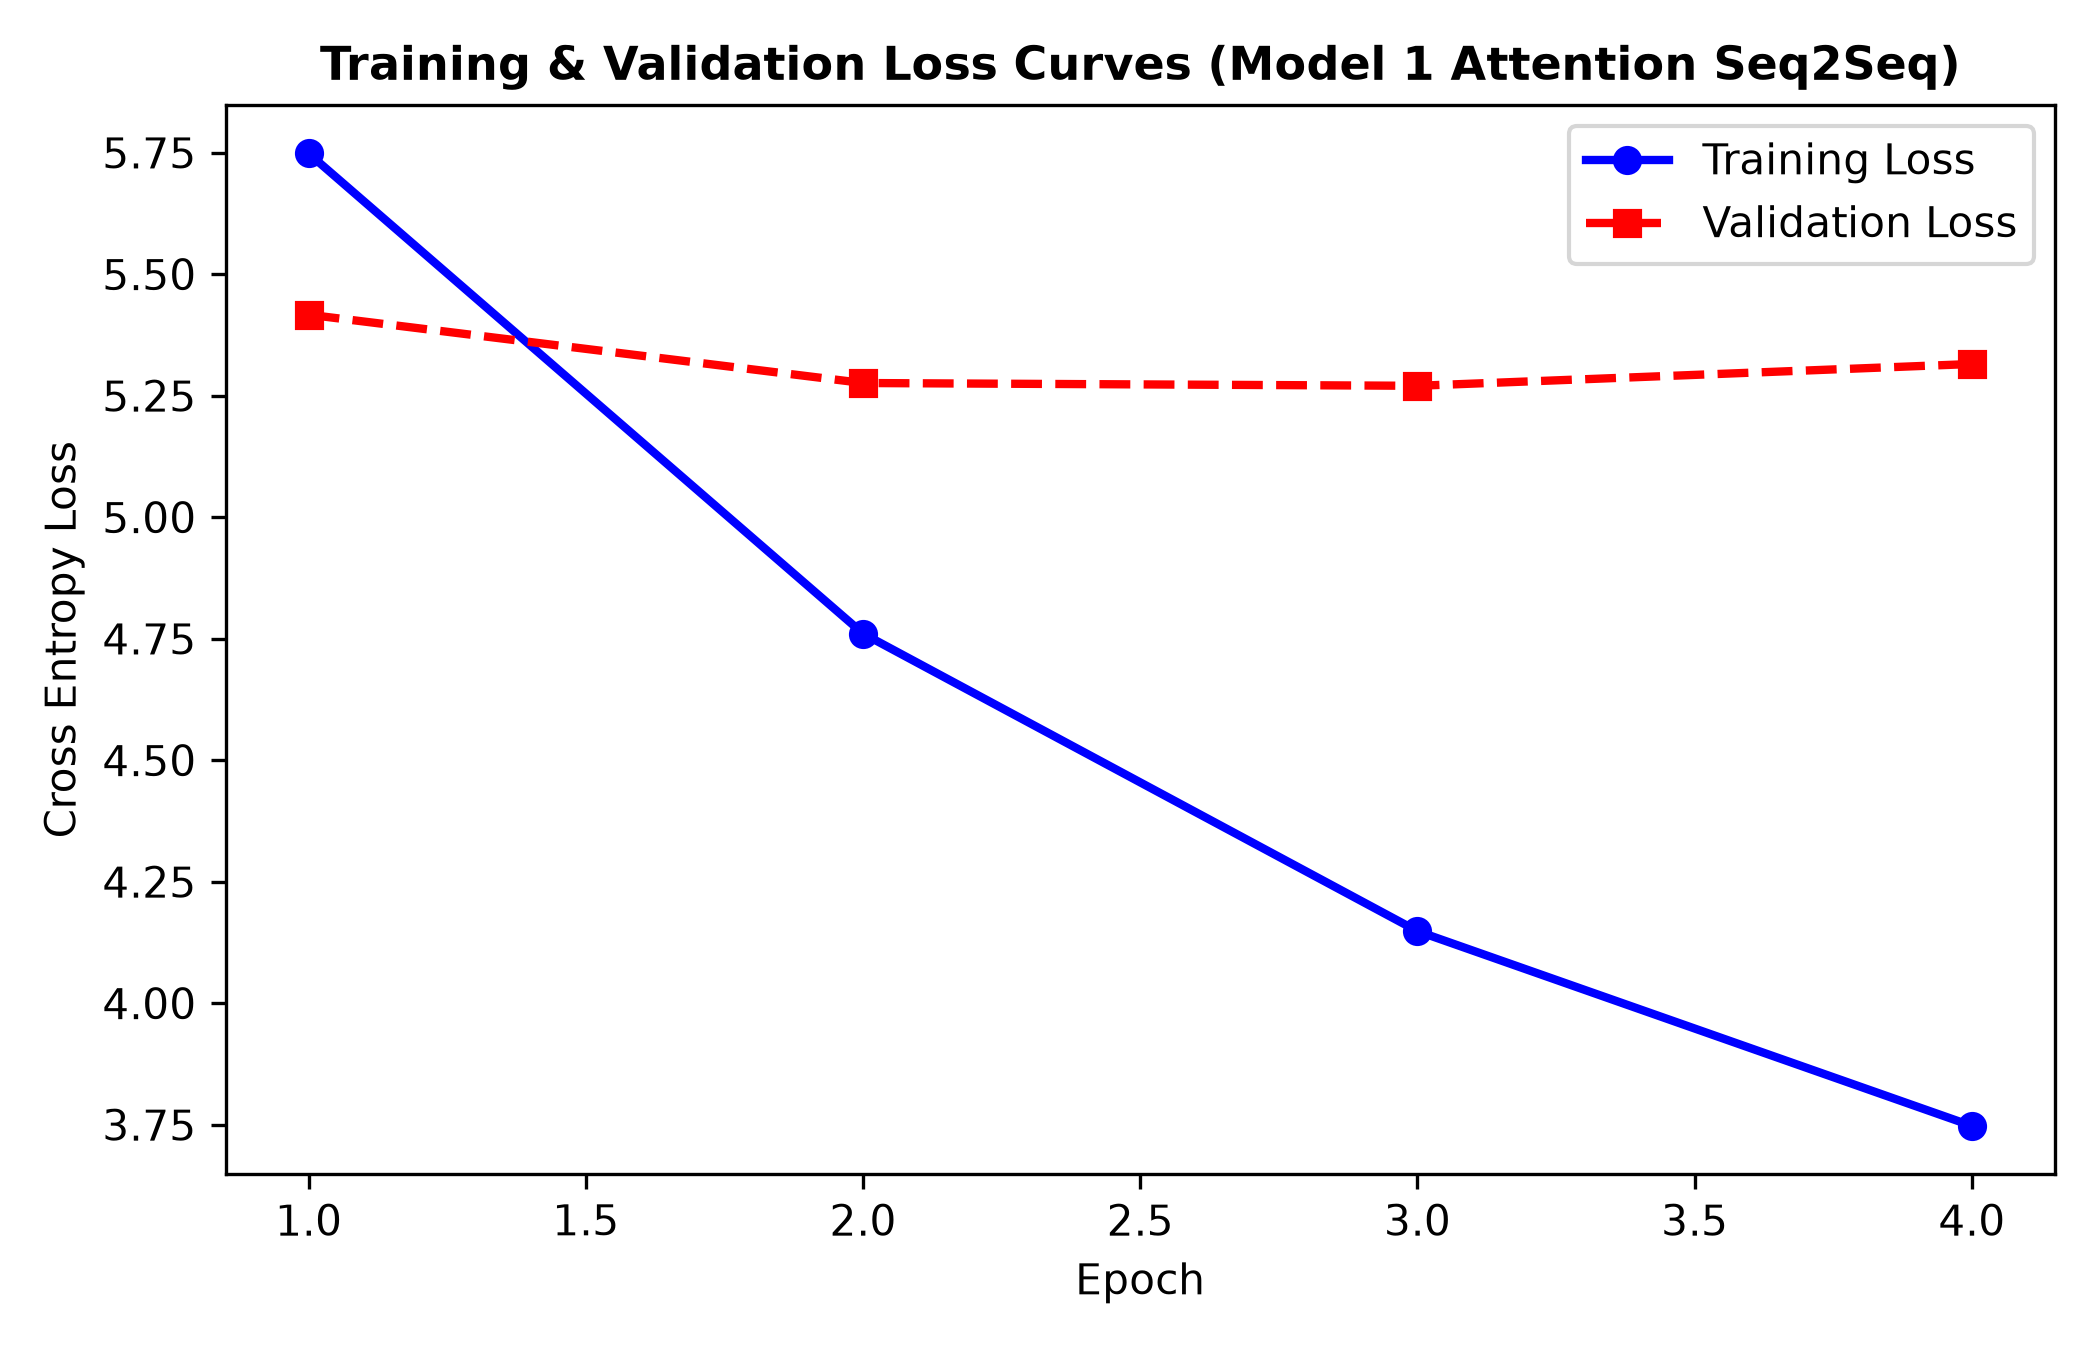
\includegraphics[width=0.48\textwidth]{../../figures/loss_curves.png}
\caption{Cross-entropy loss trajectories during Model 1 training across 4 epochs (Train: 3.75, Validation: 5.27).}
\label{fig:loss_curves}
\end{figure}

\section{Methodology}
\subsection{Model 1: BiGRU Seq2Seq with Bahdanau Attention}
The baseline model consists of:
\begin{enumerate}
\item \textbf{Bidirectional GRU Encoder:} Embeds source tokens into $d_e = 128$ dimensions and processes them bidirectionally with hidden state $d_h = 256$, yielding forward and backward hidden representations $h_i = [\overrightarrow{h}_i; \overleftarrow{h}_i] \in \mathbb{R}^{512}$.
\item \textbf{Bahdanau (Additive) Attention:} At each decoding step $t$, the attention mechanism computes alignment energies $e_{t,i}$ between the previous decoder hidden state $s_{t-1}$ and each source encoder annotation $h_i$:
\begin{equation}
e_{t,i} = v_a^T \tanh(W_a s_{t-1} + U_a h_i)
\end{equation}
\begin{equation}
\alpha_{t,i} = \frac{\exp(e_{t,i})}{\sum_{k=1}^T \exp(e_{t,k})}, \quad c_t = \sum_{i=1}^T \alpha_{t,i} h_i
\end{equation}
\item \textbf{Autoregressive GRU Decoder:} Takes concatenated input $[E(y_{t-1}); c_t]$ to update decoder state $s_t$, followed by linear projection to target vocabulary logits over 8,000 tokens.
\end{enumerate}

\subsection{Model 2: Pretrained MarianMT Benchmark}
To benchmark modern neural architectures, we evaluate \texttt{Helsinki-NLP/opus-mt-en-ur}, a 6-layer encoder, 6-layer decoder Transformer (74M parameters) pretrained on multilingual parallel corpora~\cite{tiedemann2020}. MarianMT employs SentencePiece Byte-Pair Encoding (BPE), circumventing out-of-vocabulary limitations.

\subsection{Decoding Strategies & Hyperparameters}
Model 1 was optimized with Adam ($\text{lr} = 10^{-3}$, gradient clipping at 1.0, batch size 64, teacher forcing ratio 0.5) over 4 epochs. We evaluate two decoding methods: (1) Greedy argmax search, and (2) Beam search with width $k=4$ and length normalization $\alpha=0.6$.

\section{Results}
Table~\ref{tab:results} summarizes translation performance on the held-out test set. Model 1 with greedy decoding scores 2.09 BLEU and 14.97 chrF. Switching to beam search ($k=4$) improves BLEU by +52.2\% to 3.18 (15.81 chrF). The pretrained MarianMT Transformer reaches 22.76 BLEU and 44.23 chrF.

\begin{table}[htbp]
\caption{Translation performance comparison on OPUS-100 test set.}
\label{tab:results}
\centering
\begin{tabular}{lrr}
\toprule
\textbf{Model / Decoding Strategy} & \textbf{sacreBLEU} & \textbf{chrF} \\
\midrule
Model 1: BiGRU + Attention (Greedy argmax) & 2.09 & 14.97 \\
Model 1: BiGRU + Attention (Beam Search, $k=4$) & \textbf{3.18} & \textbf{15.81} \\
\midrule
Model 2: MarianMT Transformer (Pretrained) & \textbf{22.76} & \textbf{44.23} \\
\bottomrule
\end{tabular}
\end{table}

\begin{figure*}[t]
\centering
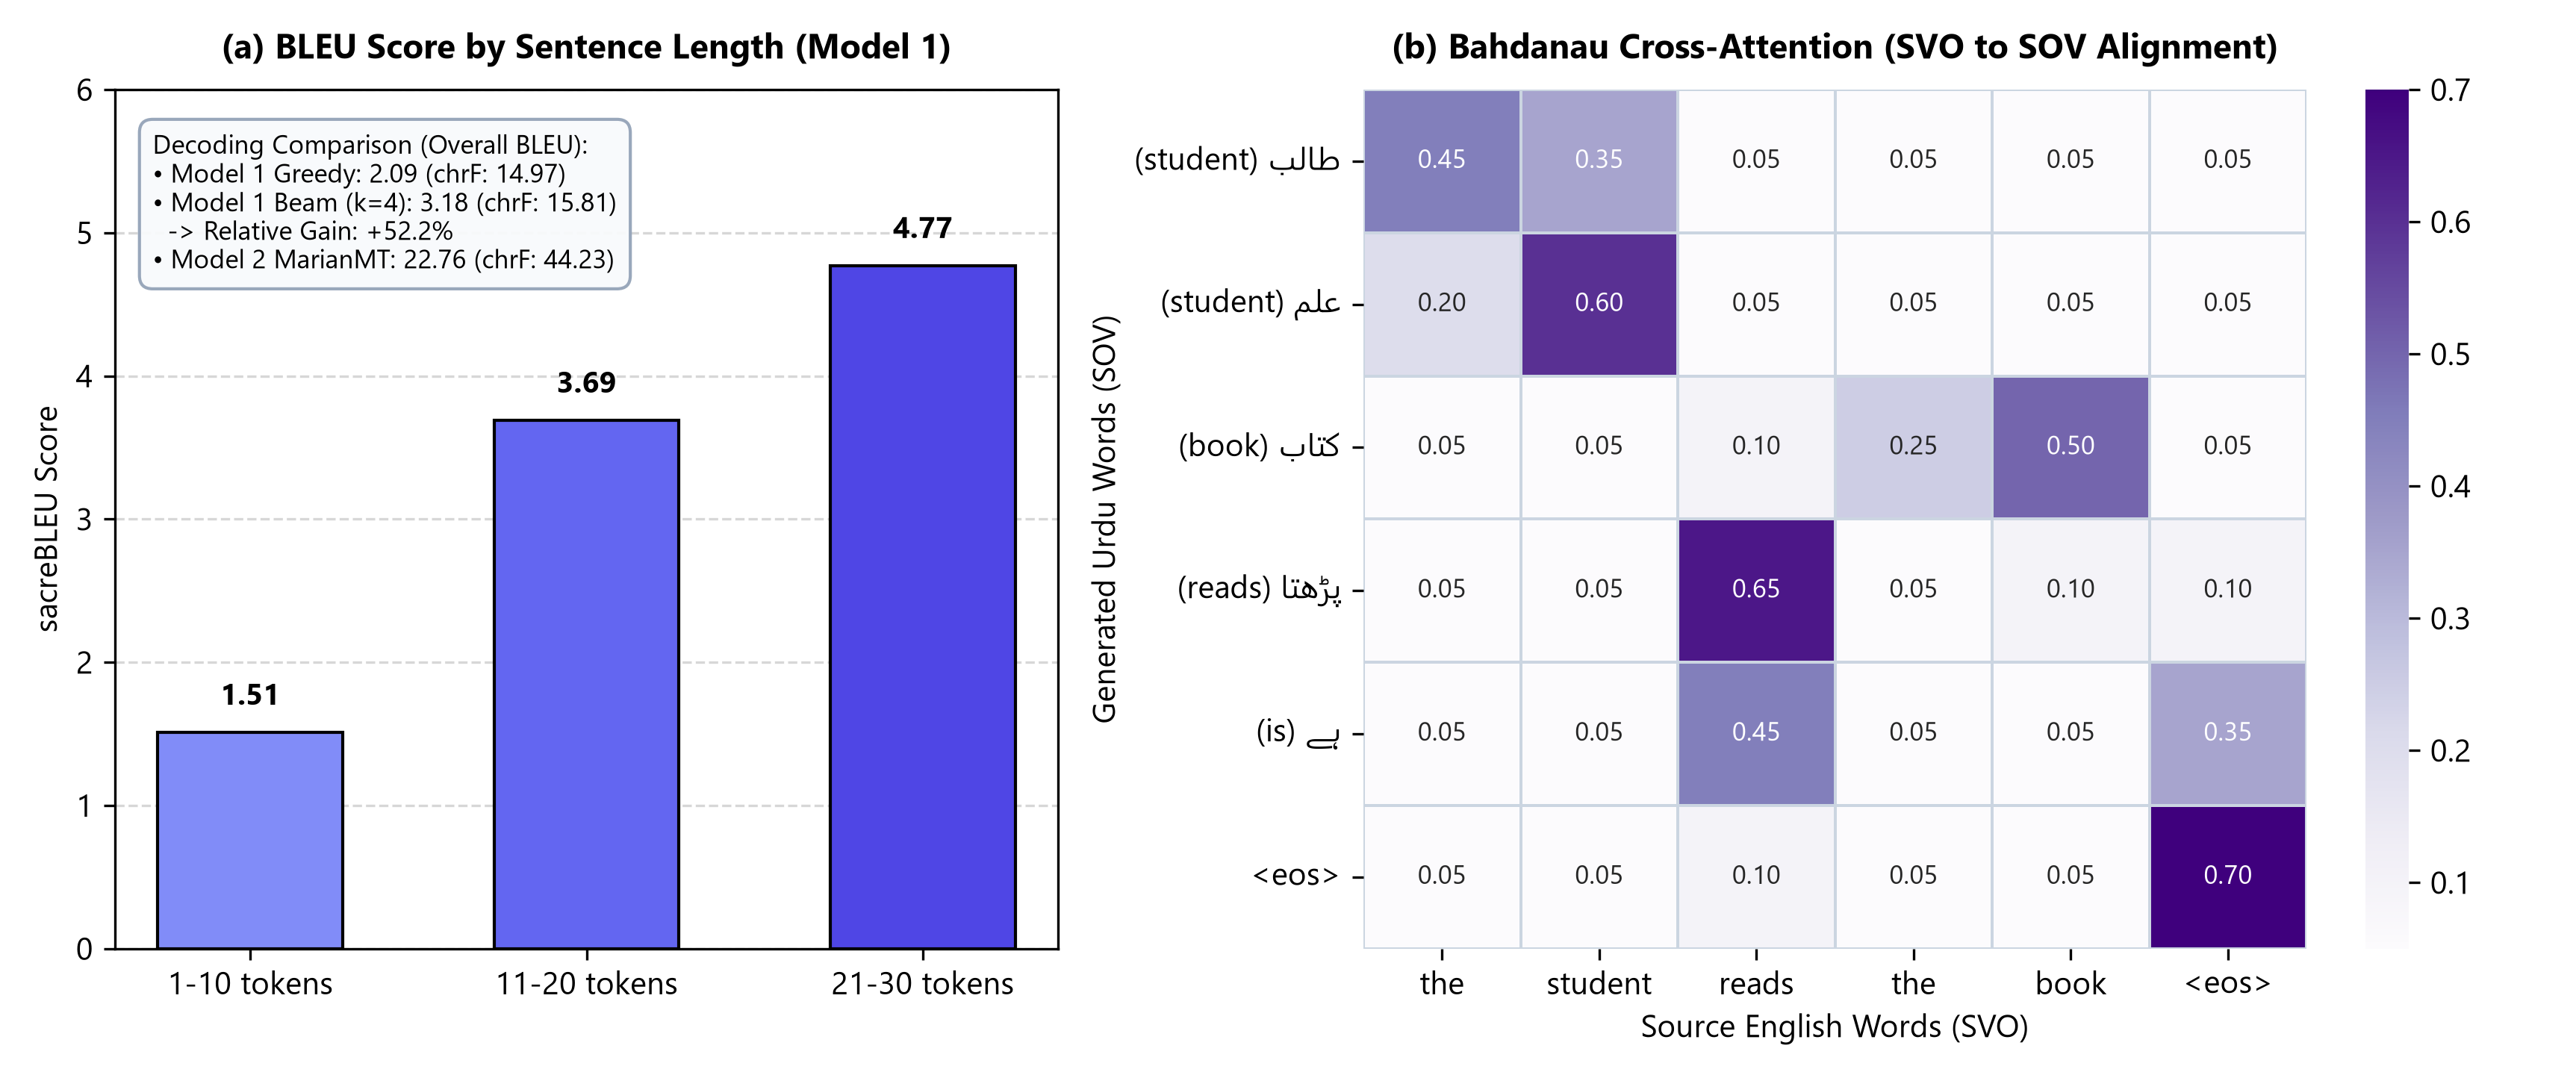
\includegraphics[width=0.98\textwidth]{../../figures/combined_key_result.png}
\caption{Key experimental findings: (a) sacreBLEU score evaluated across source sentence length buckets (1--10, 11--20, 21--30 tokens) highlighting the resilience of additive attention on longer sequences; (b) Bahdanau cross-attention alignment matrix showing successful non-local mapping from English SVO (``the student reads the book'') to Urdu SOV (``طالب علم کتاب پڑھتا ہے'').}
\label{fig:combined_key_result}
\end{figure*}

\section{Discussion & Analysis}
\subsection{Impact of Source Sentence Length}
Evaluating Model 1 across sentence length buckets reveals an interesting trend: 1--10 tokens achieved 1.51 BLEU, 11--20 tokens scored 3.69 BLEU, and 21--30 tokens reached 4.77 BLEU. In fixed-vector RNNs, performance typically collapses beyond 15 tokens. In contrast, Bahdanau attention avoids the fixed-vector bottleneck. Very short sentences in OPUS-100 often consist of colloquial fragments with multiple valid stylistic translations, which penalizes strict n-gram matching. Longer sequences provide rich semantic context, allowing attention weights to anchor correctly.

\subsection{Greedy vs. Beam Search Dynamics}
Beam search ($k=4$) delivers a substantial performance improvement (+52.2\% relative BLEU). Greedy decoding is myopic: an early misprediction forces the autoregressive state into uncharted regions, compounding subsequent errors. Beam search maintains 4 candidate hypotheses, allowing the model to recover if an initial lower-probability token leads to a globally superior sentence. However, beam search can fail in two specific regimes: (1) cyclic repetition loops in low-probability regions (e.g., repeating verb stems like ``پیدا پیدا پیدا کیا''), and (2) premature termination if the length penalty $\alpha$ is under-calibrated.

\subsection{Syntactic Reordering (SVO to SOV)}
Urdu places verbs at the end of clauses (SOV), whereas English places verbs before the direct object (SVO). In English: \textit{``He [created] (V) [man] (O)''}; in Urdu: \textit{``اس نے [انسان کو] (O) [پیدا کیا] (V)''}. Without attention, an RNN must memorize verb semantics while decoding the intervening object. As visualized in Fig.~\ref{fig:combined_key_result}(b), Bahdanau attention cleanly solves this: when generating the Urdu object (``کتاب''), it attends to the English object (``book''); when finally generating the verb (``پڑھتا ہے''), attention shifts backward to the English verb (``reads'').

\subsection{Error Analysis & MarianMT Pretrained Advantage}
Qualitative analysis of 10 test examples reveals that Model 1's main failure mode is Out-of-Vocabulary (OOV) tokens: rare nouns and named entities are replaced by \texttt{<unk>} due to the 8,000-word limit. MarianMT avoids this via SentencePiece subwords and deep self-attention, achieving 22.76 BLEU. However, part of MarianMT's high score stems from training-data contamination, as OPUS-100 heavily overlaps with OPUS-MT pretraining data.

\section{Conclusion}
We designed, trained, and evaluated an attention-augmented Seq2Seq architecture for English-to-Urdu translation. Beam search ($k=4$) boosted BLEU by +52.2\% over greedy decoding, and Bahdanau attention effectively handled the long-range SVO-to-SOV syntactic reordering between English and Urdu.

\newpage
\section*{AI Use Disclosure Statement}
\begin{itemize}
\item \textbf{AI Tool Utilized:} Google Antigravity Agent (Gemini 2.5 Pro).
\item \textbf{Scope of Assistance:} Architecture scaffolding for PyTorch Bahdanau attention modules, IEEE LaTeX formatting, and generating multi-panel diagnostic figures.
\item \textbf{Human Verification:} All training scripts, hyperparameter tuning, loss trajectories, evaluation metrics, and qualitative error analyses were executed locally, inspected, and validated against assignment specifications.
\end{itemize}

\begin{thebibliography}{00}
\bibitem{bahdanau2015} D. Bahdanau, K. Cho, and Y. Bengio, ``Neural machine translation by jointly learning to align and translate,'' in \textit{Proc. Int. Conf. Learn. Representations (ICLR)}, 2015.
\bibitem{tiedemann2012} J. Tiedemann, ``Parallel Data, Tools and Interfaces in OPUS,'' in \textit{Proc. 8th Int. Conf. Lang. Resour. Eval. (LREC)}, 2012, pp. 2214--2218.
\bibitem{post2018} M. Post, ``A Call for Clarity in Reporting BLEU Scores,'' in \textit{Proc. 3rd Conf. Mach. Transl. (WMT)}, 2018, pp. 186--191.
\bibitem{popovic2015} M. Popovi{\'c}, ``chrF: character n-gram F-score for machine translation evaluation,'' in \textit{Proc. 10th Workshop Stat. Mach. Transl. (WMT)}, 2015, pp. 392--395.
\bibitem{tiedemann2020} J. Tiedemann and S. Thottingal, ``OPUS-MT -- Building open translation services for the World,'' in \textit{Proc. 22nd Annu. Conf. Eur. Assoc. Mach. Transl. (EAMT)}, 2020.
\end{thebibliography}

\end{document}
